% last updated in April 2002 by Antje Endemann
% Based on CVPR 07 and LNCS, with modifications by DAF, AZ and elle, 2008 and AA, 2010, and CC, 2011; TT, 2014; AAS, 2016

\documentclass{llncs}
\usepackage{graphicx}
\usepackage{amsmath,amssymb} % define this before the line numbering.
\usepackage{ruler}
\usepackage[dvipsnames]{xcolor}
\usepackage{subcaption}
\captionsetup{compatibility=false}
\usepackage{xcolor}
\usepackage[width=122mm,left=12mm,paperwidth=146mm,height=193mm,top=12mm,paperheight=217mm]{geometry}
\usepackage{multirow}
\usepackage{algorithm}
\usepackage{footnote}
\makesavenoteenv{tabular}
\makesavenoteenv{table}
\usepackage[]{algpseudocode}
\newcommand{\jason}[1]{\textcolor{orange}{\textbf{JASON: #1}}}
\newcommand{\madan}[1]{\textcolor{red}{#1}}

\begin{document}
% \renewcommand\thelinenumber{\color[rgb]{0.2,0.5,0.8}\normalfont\sffamily\scriptsize\arabic{linenumber}\color[rgb]{0,0,0}}
% \renewcommand\makeLineNumber {\hss\thelinenumber\ \hspace{6mm} \rlap{\hskip\textwidth\ \hspace{6.5mm}\thelinenumber}}
% \linenumbers
\pagestyle{headings}
\mainmatter
\def\ECCV18SubNumber{1816}  % Insert your submission number here

\title{TARP: Tensorflow-based Activity Recognition Platform} % Replace with your title

\titlerunning{TARP: Tensorflow-based Activity Recognition Platform}

\authorrunning{Eric Hofesmann, Madan Ravi Ganesh, \and Jason J. Corso}

\author{Eric Hofesmann, Madan Ravi Ganesh, \and Jason J. Corso}
\institute{University of Michigan}
\newcommand{\acro}{TARP}
\newcommand{\model}{\textbf{Model Definition Block}}
\newcommand{\checkpoint}{\textbf{Checkpoint module}}
\newcommand{\metrics}{\textbf{Metrics module}}
\newcommand{\data}{\textbf{Input Data Block}}
\newcommand{\exec}{\textbf{Execution Block}}
\newcommand{\modeldef}{\textbf{Model Definition Block}}

\maketitle

\begin{abstract}
Action recognition is a widely known and popular task that offers an approach towards video understanding.
The absence of an easy-to-use platform containing state-of-the-art (SOTA) models presents an issue for the community.
Given that individual research code is not written with an end user in mind and in certain cases code is not released, even for published articles, the importance of a common unified platform capable of delivering results while removing the burden of developing an entire system cannot be overstated.
To try and overcome these issues, we develop a tensorflow-based unified platform to abstract away unnecessary overheads in terms of an end-to-end pipeline setup in order to allow the user to quickly and easily prototype action recognition models.
With the use of a consistent coding style across different models and seamless data flow between various submodules, the platform lends itself to the quick generation of results on a wide range of SOTA methods across a variety of datasets.
All of these features are made possible through the use of fully pre-defined training and testing blocks built on top of a small but powerful set of modular functions that handle asynchronous data loading, model initializations, metric calculations, saving and loading of checkpoints, and logging of results.
The platform is geared towards easily creating models, with the minimum requirement being the definition of a network architecture and preprocessing steps from a large custom selection of layers and preprocessing functions.
\acro~currently houses four SOTA activity recognition models which include, I3D, C3D, ResNet50+LSTM and TSN.
The recognition performance achieved by these models are, $XX\%$ for ResNet50+LSTM and $YY\%$ for C3D on XXXXX while I3D and TSN achieve $ZZ\%$ and $QQ\%$ on YYYYY respectively.

\keywords{tensorflow, activity recognition, framework, state-of-the-art models, C3D, I3D, Temporal Segment Networks, ConvNet+LSTM}
\end{abstract}

\section{Introduction}
\label{sec:intro}

The research community is focused on exploring concepts at the frontiers of science and helping solve problems that bog our development down.
An important part of research is the analysis of currently proposed theories and further improving upon them. 
This necessitates the use and re-use of models and theories that are currently state-of-the-art (SOTA). 
However, given the strong emphasis on concepts and modelling, coding practices are relegated to a lower priority.
Thus, there isn't a universal standard guideline for coding practice and this leads to strong variations from place to place and even between communities within a university.
Further, not all the components that are needed to re-create the results published are provided to the research community, which takes away from valuable time spent on research and instead is used to replicate the published results through common knowledge, details published in the paper and a little guesswork.
In this paper, we propose to solve this problem in the context of action recognition, in the field of computer vision.

There has been a recent positive trend towards open sourcing code in the computer vision community.
However, even when the same language is used to develop software, custom coding practices make it extremely difficult to quickly assimilate and integrate code.
When custom coding styles are combined with the vast array of languages available, e.g., tensorflow~\cite{abadi2016tensorflow}, pytorch~\cite{hdfszke2017automatic}, caffe~\cite{ijia2014caffe} in deep learning, it adds to the complexity since key words in languages tend to vary in meaning and this necessitates an extremely deep understanding of each and every language.
Subtle differences, such as, the keyword ``\texttt{\textcolor{ForestGreen}{dropout ratio}}'' can mean the ratio of nodes to drop or keep, can have massive impacts on the final results.
When put into the context of feature extraction, each deep learning language has a model zoo to access a number of staples. However, we aren't aware of such a model zoo for a task like activity recognition. 
Given the popularity of activity recognition, as a precursor to video understanding, and the prevalence of deep learning it is surprising.

We introduce \acro, which is a platform that allows the user to solely focus on the creation or fine-tuning of models by abstracting away unnecessary peripheral details like data input, computing metrics, and extracting features.
In order to avoid the complication of parsing code between different language and the complications that can arise from doing so, we use a single language, tensorflow, for our platform.
We further supplement it with a suite of SOTA activity recognition models which remove the necessity of replication and the end user can focus their time on implementing deep learning models and conduct research.

The main contributions of the platform are:
\begin{itemize}
\item Extract features from SOTA activity recognition models.
\item Quickly generate results across a combination of a variety of datasets and ANN models.
\item Single node multi-GPU expansion support to train and fine-tune models.
\item A custom input block that condenses the loading and processing of videos into a set of flexible and easy-to-use options for the user.
\item The ability to convert model weights, stored in our custom Numpy dictionary format, to alternative formats used in other deep learning languages..
\item A vast array of customized options for neural network layer definitions and preprocessing functions.
\end{itemize}

Within this report, we use the following formatting techinques,
\begin{itemize}
\item \textcolor{red}{loss} - To denote functions
\item \textcolor{blue}{file.npy} - To denote different file names
\item \texttt{\textcolor{ForestGreen}{loss\_type}} - To denote keywords in the code
\item \textbf{Model block} - To denote Blocks, submodules and any higher level construct
\end{itemize}

\begin{figure}[t!]
\centering
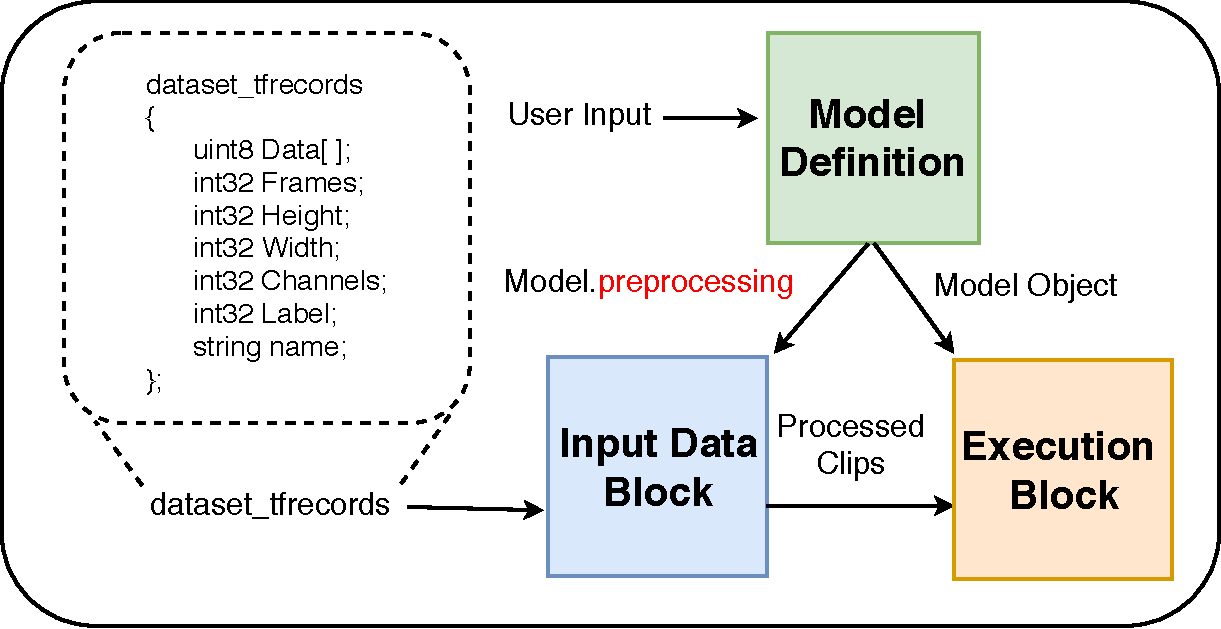
\includegraphics[width=0.8\textwidth]{images/overview.pdf}
\caption{Illustration of the three main components of \acro.
The presented color scheme will be common throught all figures in this paper.
Blue, green, and orange identify components of the \data, \model, and \exec~repectively.}
\label{fig:overview}
\end{figure}


\section{Overview of \acro}
\label{sec:overview}

As shown in Fig.~\ref{fig:overview} \acro~is comprised of three main components, 1) the \textbf{Input Data Block}, 2) \textbf{Model Definition Block} and 3) the \textbf{Execution Block}.
The \textbf{Input Data Block} processes datasets in the form of tfrecords present within in a single directory. 
The inner works of the \textbf{Input Data Block} can be divided into two simple stages,
\begin{enumerate}
\item Read video data from disk
\item Extract the desired number of clips from a given video and process them.
\end{enumerate}

The \textbf{Model Definition Block} contains functions and code that relate to the definition of a model, it's loss, data flow between different layers and the preprocessing pipeline used on input data.
On the other hand, the \textbf{Execution Block} houses all of the code required to setup, train, test as well as log the outputs of a chosen model.
This includes training the model up to a predetermined number of epochs, saving parameter values of a model are regular intervals and finally testing the performance of the trained model over a variety of recognition metrics.
The following sections provide an in depth discussion of the setup and structure of various components that make up the \textbf{Input Data}, \textbf{Model Definition}, and \textbf{Execution Blocks}.

\section{Input Data Block}
\label{sec:ipblock}
Included in the \textbf{Input Data Block} are all of the steps required to load a video and process it into the platform's desired format.
Fig.~\ref{fig:ip_block} shows the structure and flow of data as it passes through the \textbf{Input Data Block}.
The two stages of the \textbf{Input Data Block}, reading video data and extracting clips, are detailed below.

\begin{figure}[t!]
\centering
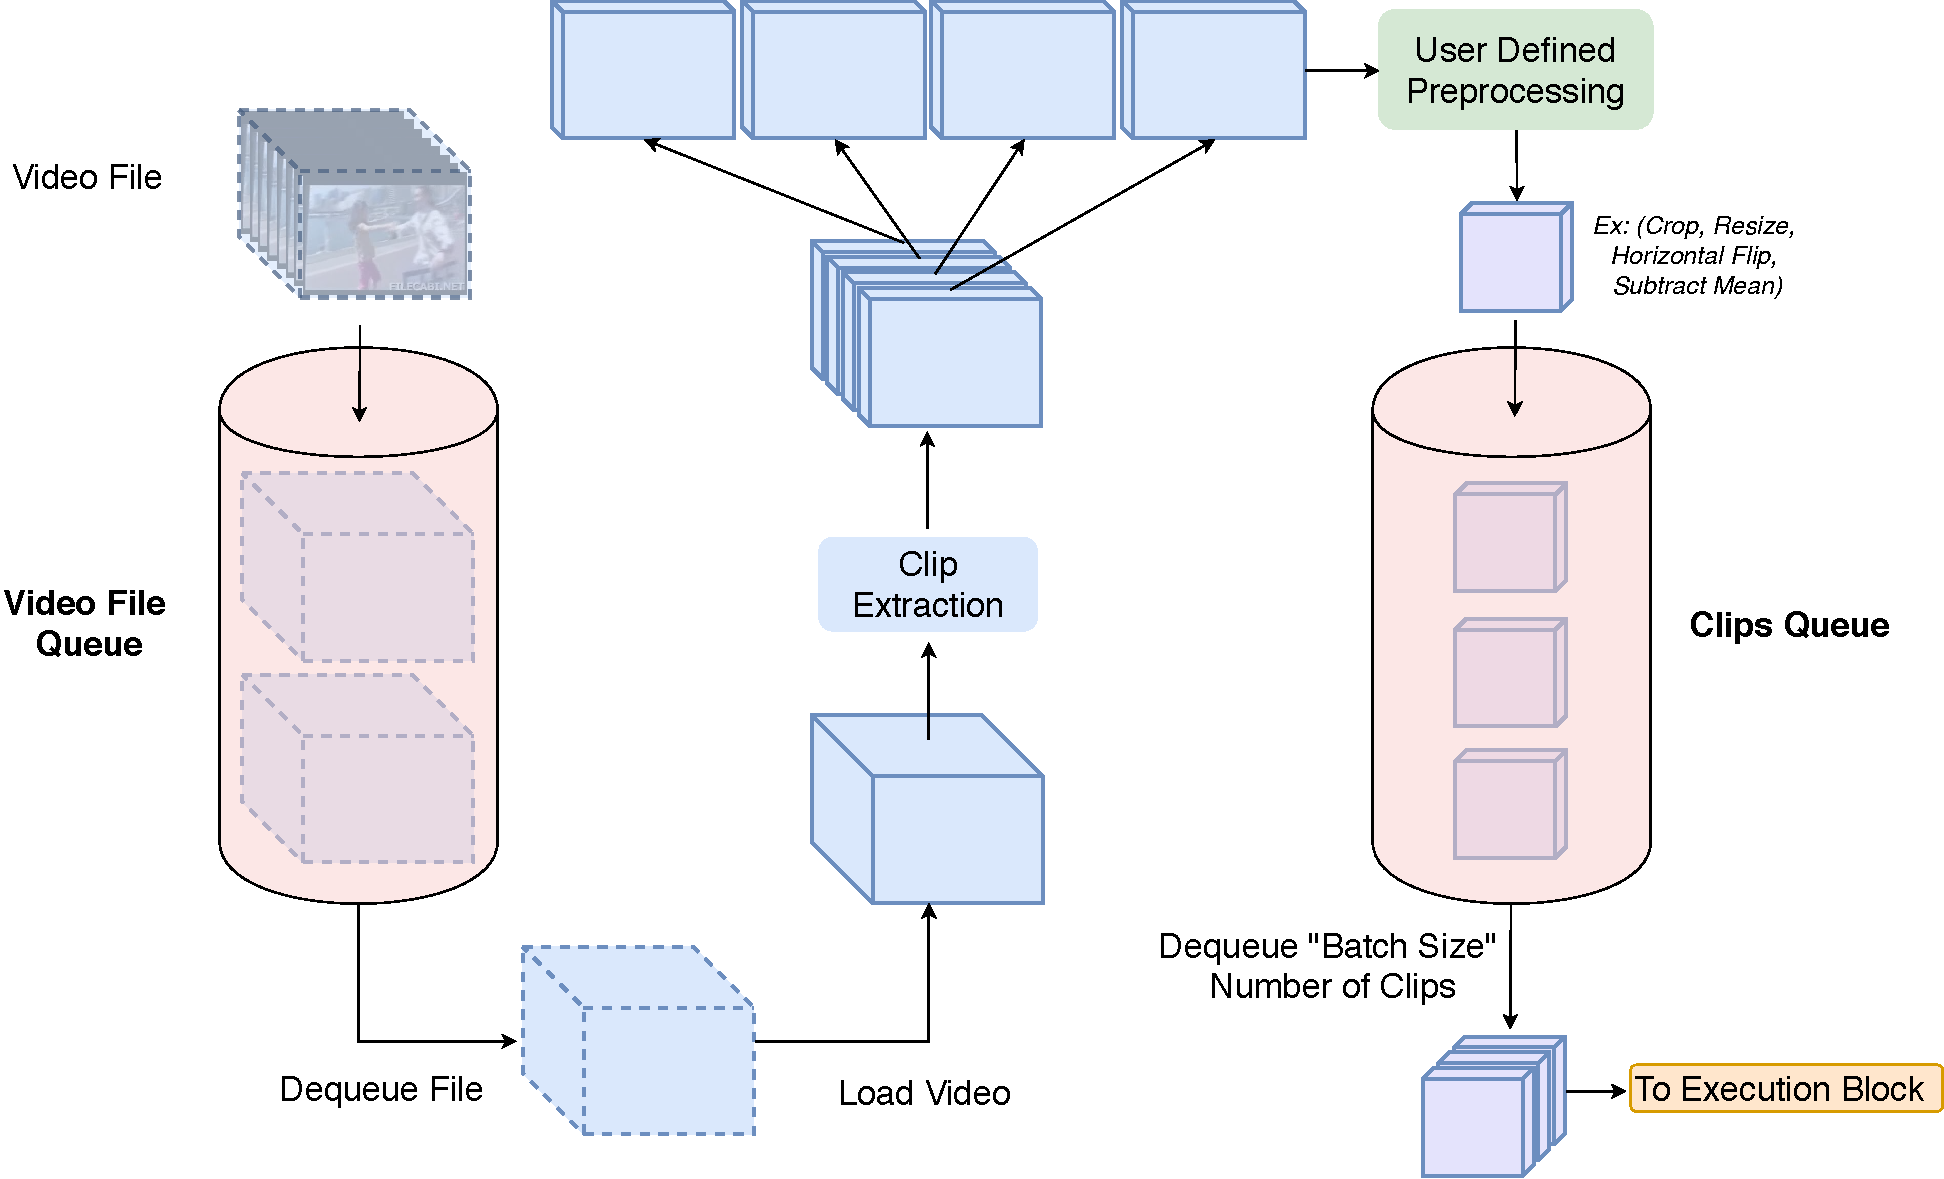
\includegraphics[width=1.0\columnwidth]{images/ip_pipeline.pdf}
\caption{This figure depicts the data flow from loading video files to passing a processed batch of clips into the specified model.
The \textbf{Input Data Block} is structured around two separate queues, one queue for storing file names of all tfrecords in the specified dataset and another queue for storing processed clips waiting to be passed to the model.
During runtime, the \texttt{\textcolor{ForestGreen}{video\_file\_queue}} gets filled with all available tfrecords filenames in a given dataset, which then get dequeued one by one.
The video corresponding to a dequeued file name gets loaded into the system and broken down into clips as described in Sec.~\ref{sec:extractclips} and Fig.~\ref{fig:extract_clips}.
Each clip then gets individually preprocessed according to a set of user defined steps as described in Sec.~\ref{sec:modeldefblock}.
The processed queues then get loaded into the \texttt{\textcolor{ForestGreen}{clips\_queue}} so that exactly one \texttt{\textcolor{ForestGreen}{batch\_size}} of clips is available to be loaded into the model.}
\label{fig:ip_block}
\end{figure}


\subsection{Read video data}
\label{sec:readdata}
In \acro, video data is stored in the form of tfrecords files to allow the entire \textbf{Input Data Block} to be constructed into the tensorflow graph for efficient parallel data loading.
These files can be generated using provided scripts and examples, assuming that the original video datasets have been acquired.
The contents of these files include the video height, width, channels, number of frames, BGR data, name of the video file, and the label of the action class related to the video as can be seen in Fig.~\ref{fig:overview}.
Video data is stored in BGR format due to the use of OpenCV~\cite{opencv_library} for converting the original video files to python arrays.
The first step of the \data~after reading in tfrecords data is to convert the video to RGB.

Reading tfrecords files is accomplished through the use of a \texttt{\textcolor{ForestGreen}{tfrecord\_file\-\_queue}} which stores the names of all tfrecords in the given dataset directory.
After a file name has been extracted form this queue, the corresponding video will then be broken down into clips and preprocessed.
To allow for the loading of multiple clips from each video, a \texttt{\textcolor{ForestGreen}{clips\_queue}} is added to the \data~to store individual clips.
These two queues work in parallel with one another, meaning that if a video is broken down into more clips than can be loaded in one \texttt{\textcolor{ForestGreen}{batch}}, the remaining clips will be stored in the clips queue.
Conversely, if the \texttt{\textcolor{ForestGreen}{clips\_queue}} does not contain enough clips to fill one \texttt{\textcolor{ForestGreen}{batch}}, then the \texttt{\textcolor{ForestGreen}{tfrecord\_file\_queue}} will automatically load and process a new video.
Due to this variablity, the implementation of the \texttt{\textcolor{ForestGreen}{clips\_queue}} is critical.

Note: When loading the dataset HMDB51, videos are stored in a 30 frames-per-second (fps) format while most models require 25 fps. A function, \textcolor{red}{\_reduce\_fps} is used to remove every sixth frame from HMDB51 videos in order to reduce the fps.


\begin{figure}[t!]
\centering
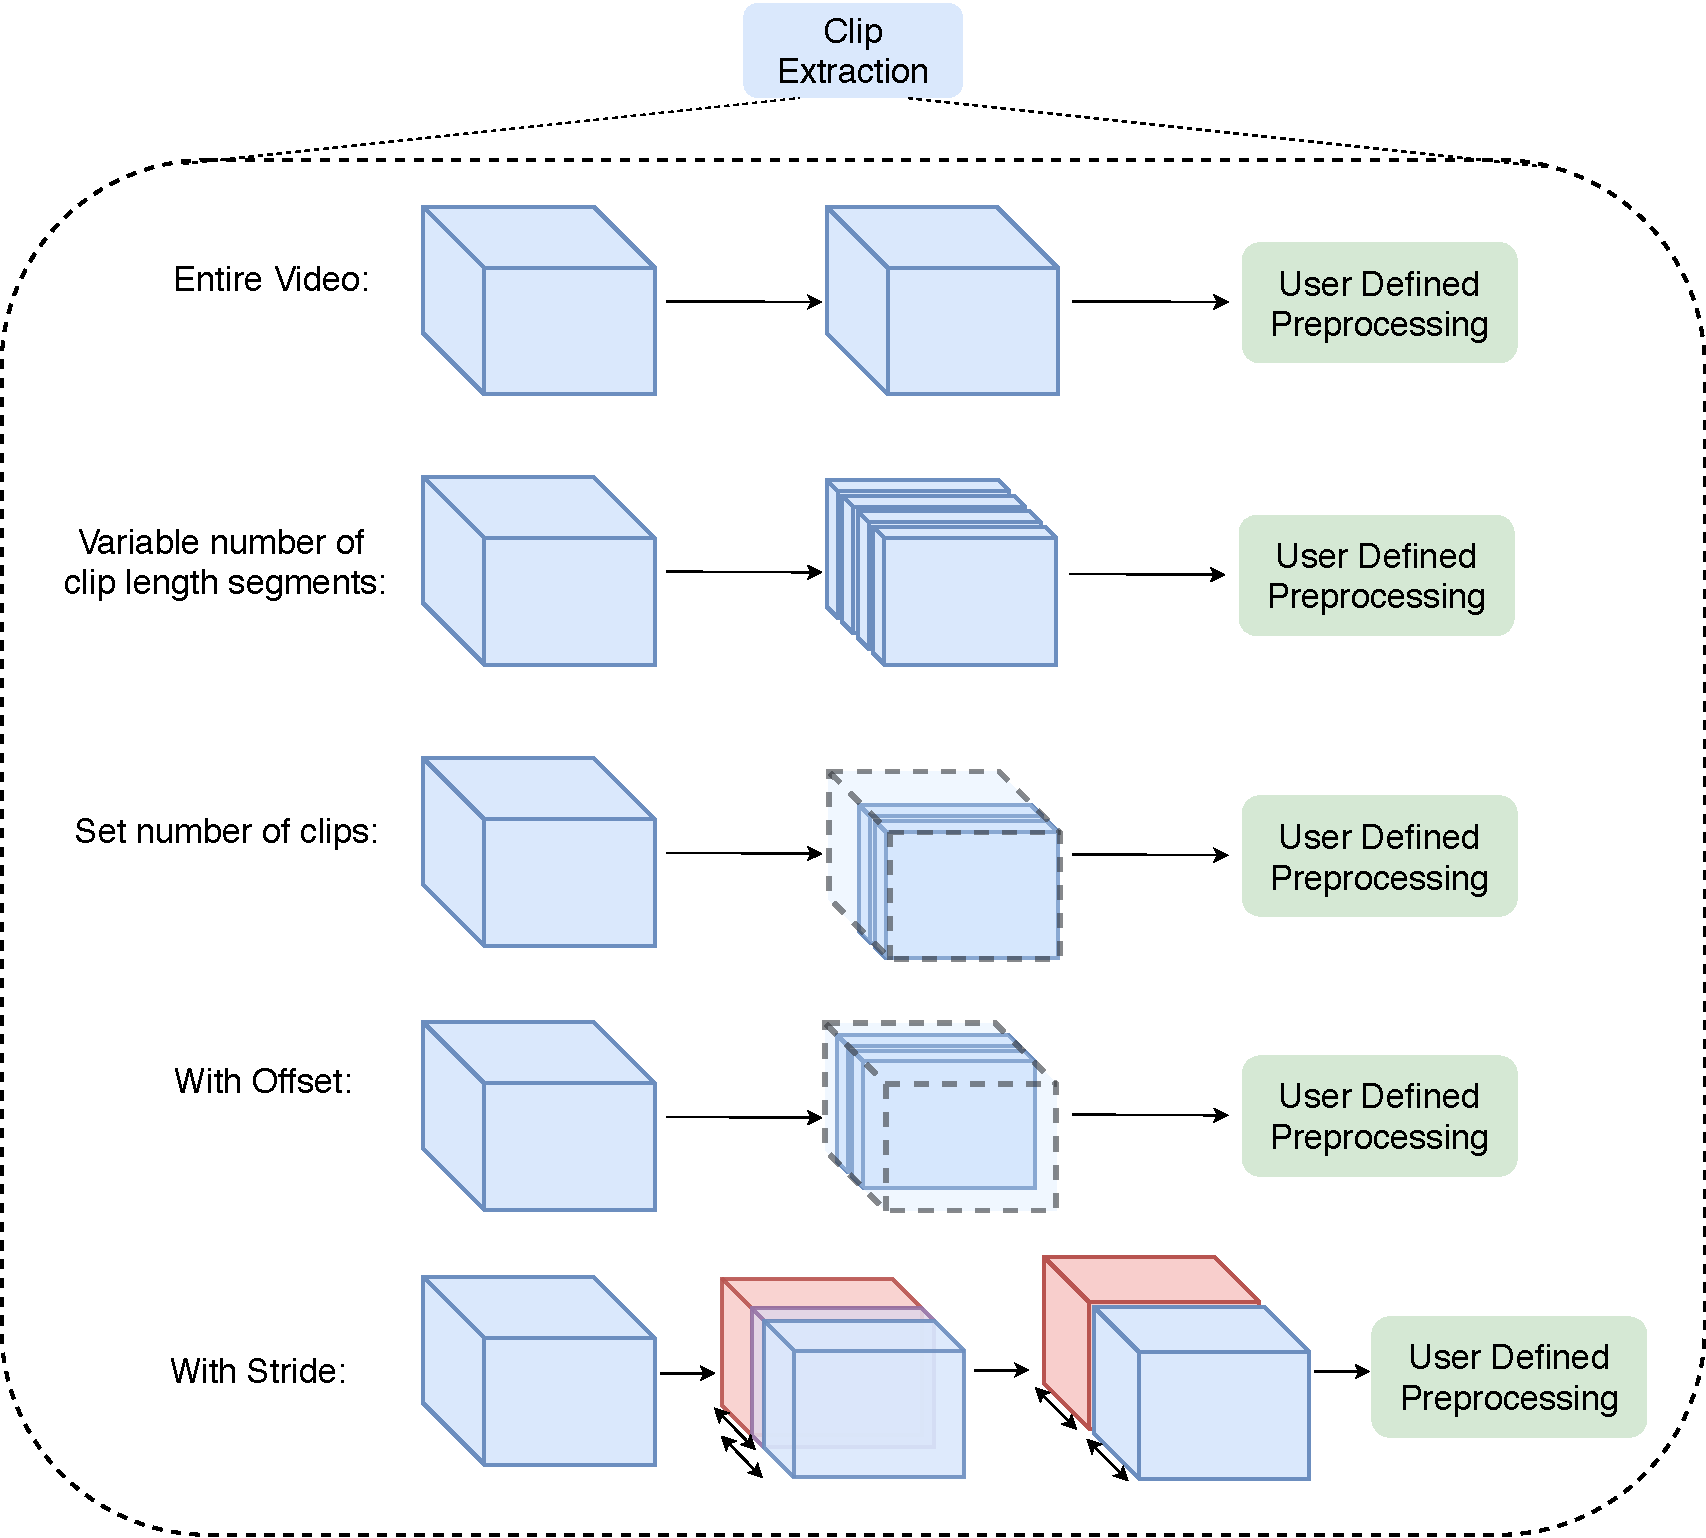
\includegraphics[width=0.8\columnwidth]{images/extract_clips.pdf}
\caption{This figure shows the various ways that a video can be broken into clips.
By default the entire video is passed directly on to the user defined preprocessing without any modifications.
A variable number of clips can be extracted from a video if only the \texttt{\textcolor{ForestGreen}{clip\_length}} parameter is given.
Alternatively, a set number of clips of a certain length can be extracted from every video using the \texttt{\textcolor{ForestGreen}{num\_clips}} parameter.
If a video does not contain enough frames to extract the requested number of clips, the video will be looped until the necessary frame count is reached.
There also exists an \texttt{\textcolor{ForestGreen}{offset}} parameter which can be set to randomly modify where from the beginning of the video the function begins to extract clips. 
The \texttt{\textcolor{ForestGreen}{stride}}  parameter can be used to set a number of frames that will be common between sequential clips.
This \texttt{\textcolor{ForestGreen}{stride}} parameter can be set to a negative value to skip a set number of frames between sequential clips.
}
\label{fig:extract_clips}
\end{figure}

\subsection{Extract clips}
\label{sec:extractclips}
Certain models, for example C3D~\cite{6165309}, require their inputs to be in the form of multiple clips extracted from a single video.
Fig.~\ref{fig:extract_clips} details the various methods of breaking down a video into clips.
The methods shown can be used in conjunction with one another to give the user the flexibility needed to extract clips with different dimensions.
All of this can be done through the use of only a handful of arguments including, \texttt{\textcolor{ForestGreen}{clip\_length}}, \texttt{\textcolor{ForestGreen}{num\_clips}}, \texttt{\textcolor{ForestGreen}{clip\_offset}}, and \texttt{\textcolor{ForestGreen}{clip\_stride}}.
By default, the clip extraction algorithm is set to process an entire video at a time and only extract clips if the required arguments have been specified.
In addition to the options shown in Fig.~\ref{fig:extract_clips}, \acro~also provides an option for random clip selection.

Once clips have been extracted, they are preprocessed using a selected model's preprocessing pipeline.
The desired preprocessing file for a model can be defined within the \textbf{Model Submodule} and it is used automatically in the \textbf{Input Data Block}.
Preprocessed clips can significantly vary in shape when compared to the input video.
Any change in frame height, width, or number of frames is allowed as long as the number of input and output dimensions of a clip are retained.
The \texttt{\textcolor{ForestGreen}{clips\_queue}} is designed to be compatible with the shape [\texttt{\textcolor{ForestGreen}{input\_dimensions}}, \texttt{\textcolor{ForestGreen}{size}}, \texttt{\textcolor{ForestGreen}{size}}, \texttt{\textcolor{ForestGreen}{sequence\_length}}] for the entirety of a training or testing session.

Note: Due to the nature of tensorflow enqueue operations, errors that occur within an enqueue operation do not throw an appropriate error message.
The enqueue is simply canceled and an error will occur when the dequeue attempts to access an empty queue.
For example, this effect can be seen if an error occurs in the user defined preprocessing submodule.
In order to allow proper debugging of the preprocessing submodule, the argument \texttt{\textcolor{ForestGreen}{preprocDebugging}} is available to bypass the \texttt{\textcolor{ForestGreen}{clips\_q}} and see any error stack tracebacks.
Since the queue used to store clips is removed, the requirement is set that \texttt{\textcolor{ForestGreen}{batch\_size}} must equal \texttt{\textcolor{ForestGreen}{num\_clips}} while debugging.



\section{Model Definition Block}
\label{sec:modeldefblock}

\begin{figure}[b!]
\centering
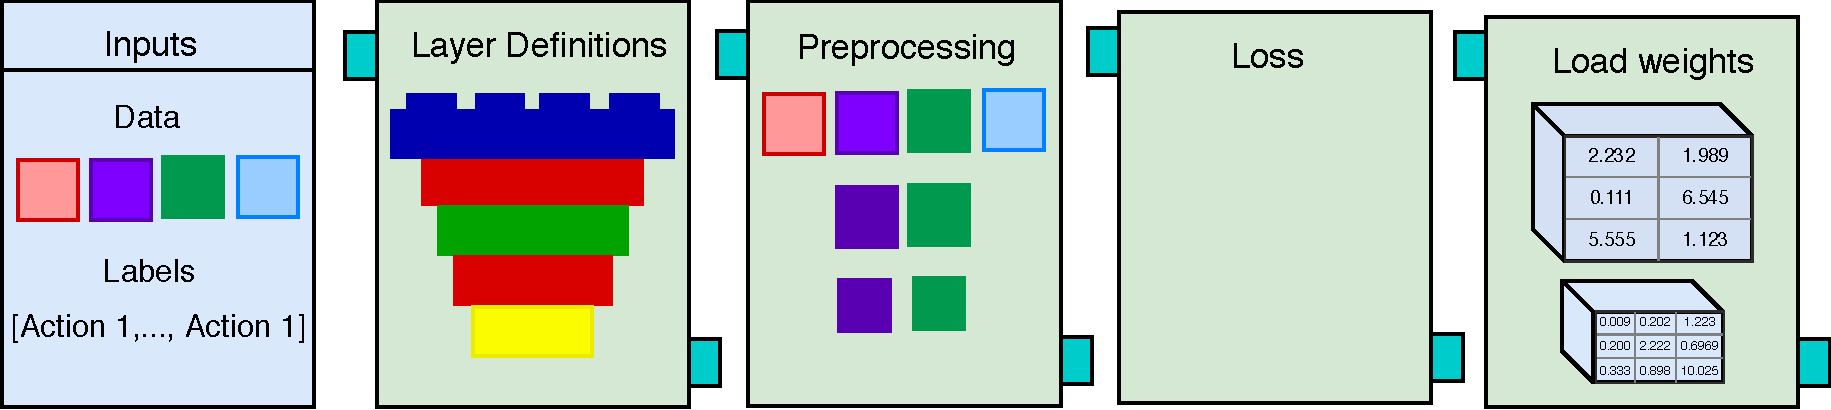
\includegraphics[width=\columnwidth]{images/model_submodule.pdf}
\caption{The components of the \modeldef: 1) Preprocessing, 2) Layer definitions, 3) Loss, and 4) Loading weights, are shown in green.
These four modules are to be implemented by the user when creating a new model. }
\label{fig:model_submodule}
\end{figure}


\subsection{Preprocessing}
The class definition of a model within \acro~can be divided into four main components as shown in Fig.~\ref{fig:model_submodule}.
Preprocessing is the first module in the \model~that gets used within \data.
Activity recognition models employ a variety of preprocessing methods on a frame or clip-based level for data augmentation.
These can include frame-wise cropping, flipping, and resizing, or clip-wise cropping, flipping, temporal offsets, resampling, looping, and more.
In keeping with the modular design paradigm, we use individual functions to define each variant of the preprocessing block.
An entire preprocessing pipeline and multiple variants of such pipelines are defined within a file marked with the suffix ``\textcolor{blue}{\_preprocessing.py}''. 
This is done to increase their reusability and ensure debugging them is easy.
Within the class definition of a model, multiple preprocessing pipelines can be included using a simple \textit{if-else} construct in conjunction with the \texttt{\textcolor{ForestGreen}{preproc\_method}}.
The expected final product from any preprocessing function is the complete preprocessed input data that needs to be passed into a network's input layer.

\subsection{Model Architecture}
The definition of a model's input layer and the subsequent layers that make up the model's network architecture should be present within the \textcolor{red}{inference} function.
The layers used must strictly be called from within the set of definitions provided within the \textcolor{blue}{layer\_utils} file.
This ensures that layer definitions are not specific to any network and become available to all models defined within \acro.
Further, it is essential that the inference function returns the outcome of any and all desired layers from within the defined network.
Any accompanying functions to help quickly and/or recursively define a network can be added outside of the inference function.


\subsection{Loss and Loading Weights}
As a minor deviation from standard practices, we attach the definition of a loss to a model instead of the main training file.
We do this to avoid cluttering and increasing the complexity of the main training file.
Thus, a prime requirement within any model definition is the implementation of a loss function, with the expected return from this function being the final loss value.
To add further flexibility in using multiple losses with a single model, the basic loss function can be overloaded to call different losses using the internally defined \texttt{\textcolor{ForestGreen}{loss\_type}} keyword.

The final and optional component of any model definition within \acro~is the definition of the \textcolor{red}{load\_default\_weights} function.
This function is defined to ensure that a predetermined set of weights can be loaded into a network's layers.
The explicit rules required to define the layer names and ensure their respective weights can be assigned are provided in Section~\ref{sec:checkpoint}.
The final values returned by this function are the parameter weights loaded from an external numpy file.

\subsection{Automatic Template Generation}
Given that the focus of \acro~is to help the end-user quickly define and integrate a model to the framework, we provide a template file named \textcolor{blue}{models\_template.py} which provides the outline for the user to quickly fill out the inference, preprocessing, loss and load weights functions.
A separate file named \textcolor{blue}{models\_preprocessing\_template.py} provides an outline of the necessary functions to define the preprocessing pipeline.
Once a model has been completely defined, it is automatically imported into the framework through a recursive call strategy.
To quickly track and log a model class variable an inbuilt dictionary named \texttt{\textcolor{ForestGreen}{track\_variables}} is available.
Adding any pre-defined variable name and graph title allows the logging of the desired variable on tensorboard.

Note: 1) Any model defined must be placed within the models folder under a directory with the same name as that of the model,
2) The actual model file must be named with a suffix ``\textcolor{blue}{\_model}''.
2) No explicit model class attributes can be added to a specific model. Instead, they must be added to the \textcolor{blue}{model\_abstract.py} file and made available to any and all model definitions within \acro.

The models that come standard with \acro~include SOTA activity recognition architectures I3D~\cite{carreira2017quo}, C3D~\cite{6165309}, ResNet50~\cite{He2015}, and TSN~\cite{wang2016temporal}.




\section{Execution Block}
\label{sec:execblock}
The \textbf{Execution Block} forms the largest component of the entire platform. 
Its code can be broken down into parts that are used during two alternate phases, training and testing.
Fig.~\ref{fig:exec_block} illustrates this concept and highlights the modules used within each phase.
An algorithmic overview of each phase, followed by a detailed description of the various modules used within them are provided in the following sections.

\begin{figure}[t!]
\centering
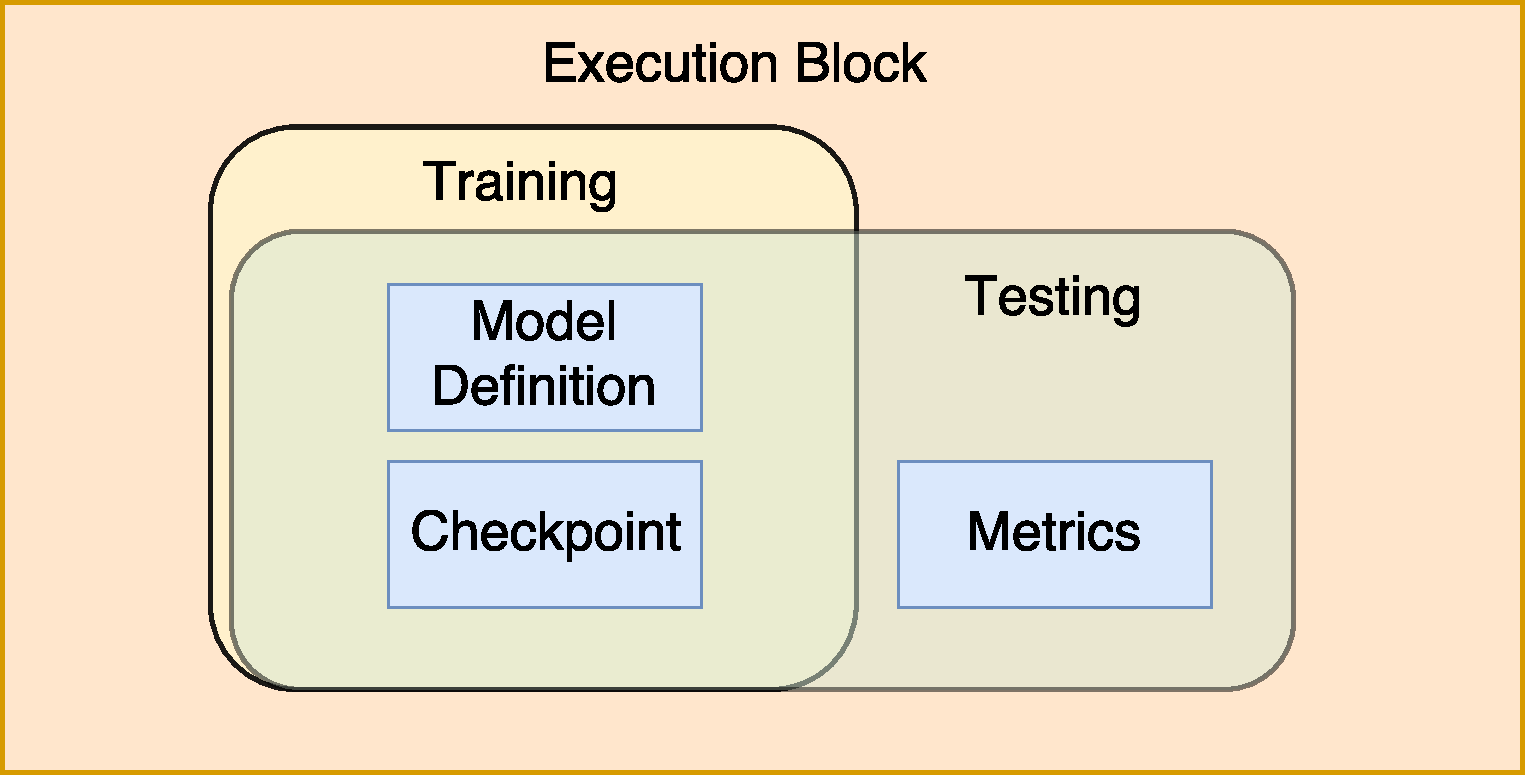
\includegraphics[width=0.8\columnwidth]{images/exec_block.pdf}
\caption{Training and Testing are the two major phases within the execution block. Checkpoint-based functions are part of both phases while metrics are calculated during the testing phase, after models are trained.}
\label{fig:exec_block}
\end{figure}

\subsection{Training: Flow of processes}
\label{sec:training}
Training, within the context of the execution block, follows the process flow outlined in Alg.~\ref{}.
The beginning of every training phase is associated with the selection and set up of a model.
Basic model parameters such as input/output data dimensions, batch normalization, dropout rate, and etc. are passed into the \model~for this purpose.

Once the model has been set up, the next step is to ensure that the parameter weights for the chosen model are retrieved.
If the model has been pre-trained using \acro~and the user desires to further fine-tune the model, then the model parameter's weights from the latest checkpoint will be restored.
By default, the standard pre-trained weights are loaded into the model.
Alternatively, a random initialization option, for users to train a model from scratch is also provided.
As a backup when a specified checkpoint is unavailable, the system defaults to the random intialization option, with an additional warning provided to the user about the setup being used.

After the preparation of the model is complete, data tensors are retrieved from the \data~ and interfaced to the model.
The main data retuned from \data~are the video frames, their corresponding labels and video names.
With the availability of the model and data, the next step is to create a copy of the model on each of the selected number of GPUs within a compute node.
Within each GPU, the inference function of \model~is used to generate a copy of the layer definitions.
Here, the variable names are re-used to ensure that the same copy of weights are associated throughout all the GPUs.
\acro~only supports the extension of a model within a compute node of a cluster.
Currently, it cannot be distrbute a model across mutiple nodes or split a model across multiple GPUs within a node.

From each of the model copies, we retrieve a desired layer's output.
Given that the most common approach to training a network is through the use of logits returned from the final layer, we use the variable logits, associated with the last layer, to obtain a loss value.
Finally, the loss and gradients, computed from the loss, across all the model copies are accumulated into the loss\_array and gradients\_array respectively.
The contribution of each model copy is weighted equally and the final gradient used to update the weights of the model is obtained by taking the average of values stored in the gradients\_array.
This the final stage in the definition of the tensorflow graph required for training.

\begin{algorithmic}[H]
\Procedure{Training}{}
\State \textbf{Model\_Definition\_Block}.\textcolor{red}{setup}(model\_params)
\State \textbf{Checkpoint}.\textcolor{red}{load\_param\_weights}(default or specific file)
\State Data, Labels = \textbf{Data\_Input\_Block}.\textcolor{red}{load\_data}(expt\_params)
\\
\For{each GPU within given node}
\State \textbf{Model\_Definition\_Block}.\textcolor{red}{inference}(Data, model\_params)
\State tower\_loss = \textbf{Model\_Definition\_Block}.\textcolor{red}{loss}(Labels, returned\_logits)
\State tower\_gradients = gradients(tower\_loss)
\State loss\_array.store(tower\_loss)
\State gradients\_array.store(tower\_gradients)
\EndFor
\\
\State grad = average\_gradients(gradients\_array)
\State train\_op = apply\_gradients(grad)
\\
\While{no\_videos\_loaded \textless~(total\_epochs $\times$ videos\_in\_dataset)}
\State \textbf{Checkpoint}.\textcolor{red}{save}() @ regular intervals
\State sess.run(train\_op)
\State update(no\_videos\_loaded)
\EndWhile
\EndProcedure
\end{algorithmic}

After the tensorflow graph for training has been defined, the next step is to execute the graph.
Usually, models are trained for a typical number of epochs, iterations over the entire dataset.
Within each epoch, based on a set frequency of iterations, we save the model parameter's weights using \checkpoint.save().
The main operation that gets executed within each iteration is the training operation that links the calculation of losses, gradients and their application.
It is important to note that during the setup of the experiment, \acro~ offers adaptive learning rate control which steps down the learning rate when the training loss plateaus.
The repeated application of train\_op forms the most crucial and final step in the training process flow.



\subsection{Testing: Flow of processes}
\label{sec:testing}

Testing begins similarly to training in that the specified model gets defined and initialized according to the \modeldef.
After a model object has been instantiated, the model weights are loaded.
There is an option to either load the weights from the default weights file specified within the \modeldef or to initialize the model to random weights.
Most commly, however, the \checkpoint is used to load the weights of a model that has been trained from scratch or fine-tuned within \acro.

Once the model weights are accessible, the dataset will be loaded into the system following the process described in the \data in Sec.~\ref{sec:ipblock}.
The shape of input data is set to allow for any number of different videos or clips to be loaded for testing within a single \texttt{\textcolor{ForestGreen}{batch}}.
This is useful in C3D for example, where a consensus across the outputs for multiple clips is calculated which will act as the prediction for an entire video.

Before data can be loaded into the model, the model must first be copied onto the GPU.
While only a single GPU is used for testing, a ``Device ID'' list can still be given to \acro~to determine the correct GPU to be used.
If the list contains more than one GPU Device ID, the first element in that list will be used.
The process of copying the model to the GPU is based around calling \textbf{Model\_Definition\_Block.}\textcolor{red}{inference} in the scope of each ID.

The \textbf{Model\_Definition\_Block.}\textcolor{red}{inference} call will return the output of the layer specified in the \texttt{\textcolor{ForestGreen}{return\_layer}} argument.
By default, the \texttt{\textcolor{ForestGreen}{logits}} layer is returned by \textcolor{red}{inference} and it is of the shape [\texttt{\textcolor{ForestGreen}{batch\_size}}, \texttt{\textcolor{ForestGreen}{sequence\_length}}, \texttt{\textcolor{ForestGreen}{output\_dims}}].
In general, a softmax function is applied whenever \texttt{\textcolor{ForestGreen}{logits}} are returned.
However, the application of softmax can be removed using the \texttt{\textcolor{ForestGreen}{useSoftmax}} argument.
With the model output acquired, the final steps of preparation for testing is to set up the output directory structure (\metrics~detailed in Sec.~\ref{sec:metrics}), and to load weights into the model (\checkpoint in Sec.~\ref{sec:checkpoint}).

The testing block iterates through the \texttt{\textcolor{ForestGreen}{num\_vids}} specified, which generally includes an entire testing split of a dataset.
Within each iteration, the tensorflow session is run to extract the model's \texttt{\textcolor{ForestGreen}{output\_predictions}}, ground truth \texttt{\textcolor{ForestGreen}{labels}}, and all video \texttt{\textcolor{ForestGreen}{names}} in the current batch.
If the \texttt{\textcolor{ForestGreen}{avg\_clips}} argument has been specified, then the \texttt{\textcolor{ForestGreen}{output\_predictions}} are averaged over their first dimension, which is the number of clips loaded for this testing iteration.
A tracker counts the number of videos that have been loaded using the video \texttt{\textcolor{ForestGreen}{names}} output.
The \texttt{\textcolor{ForestGreen}{output\_predictions}} and ground truth \texttt{\textcolor{ForestGreen}{labels}} are then fed into the \metrics for logging and storage.

\begin{algorithmic}[H]
\Procedure{Testing}{}
\State \textbf{Model\_Definition\_Block}.\textcolor{red}{setup}(model\_params)
\State \textbf{Checkpoint}.\textcolor{red}{load\_param\_weights}(default or specific file)
\State Data, Labels = \textbf{Data\_Input\_Block}.\textcolor{red}{load\_data}(expt\_params)
\\
\For{one GPU}
\State \textbf{Model\_Definition\_Block}.\textcolor{red}{inference}(Data, model\_params, return\_layer)
\If{use\_softmax}
\State logits = softmax(logits)
\EndIf
\EndFor
\\
\State \textbf{Metrics}()
\\
\While{num\_videos\_loaded \textless~videos\_in\_dataset}
\State output\_predictions = sess.run(logits)
\If{average\_over\_clips}
\State mean(output\_predictions, axis=0)
\EndIf
\State \textbf{Metrics.}\textcolor{red}{log\_prediction}(output\_predictions)
\State update(num\_videos\_loaded)
\EndWhile
\EndProcedure
\end{algorithmic}

Once all videos have been tested, the thread coordinator for the input queues is stopped and the all predictions from the \metrics are saved in a numpy format.

\subsection{Checkpoint Module}
\label{sec:checkpoint}
The \checkpoint contains utility functions that handle all the essential operations w.r.t. checkpoints.
Checkpoints themselves are stored in a custom format as shown in Fig.~\ref{fig:checkpoint_recursive}.
This format readily lends itself to a recursive access strategy while offering easy conversion capabilities from its native numpy format to ``\textcolor{blue}{.ckpt}'',``\textcolor{blue}{.caffemodel}'' and other formats.
Among the variety of operations that can be performed on and using checkpoints, there are two broad categories, Load/Save and Tensor handling.

\paragraph{Load/Save}
At the beginning and end of every training processes, the ability to save and recover the current/last known state of the model parameters is paramount.
In order to save the current state of a model's parameters, a new checkpoints folder is generated in the results directory.
The folder structure generated to save the checkpoints is, \textless dataset\textgreater/\textless preprocessing\_method\_name\textgreater/\\\textless experiment\_name\textgreater/\textless metric\_name\textgreater/checkpoints.
Within this folder three distinct files are generated.
\begin{itemize}
\item Checkpoint file: A replica of the checkpoint file obtained from native tensorflow code is generated by the \textcolor{red}{save\_checkpoint} function.
The current global step is saved within this file, named ``\textcolor{blue}{checkpoint}''.
\item Data file: A separate data file is used to store the current learning rate of the experiment.
The file is named using the convention \textcolor{blue}{checkpoint-\textless global step number\textgreater .dat}.
\item Numpy weights file: Variables declared and available within the global scope of the experiment are retrieved, name and value, and stored within the numpy weights file.
It follows a similar naming convention to the Data file, \textcolor{blue}{checkpoint-\textless global step number\textgreater .npy}.
\end{itemize}

When a checkpoint is being loaded, the utility searches for each of the three files defined above to each return a distinct variable holding the contents of the files.
If any of the files are missing, the checkpoints fails to get loaded and it is a clear indication of a corrupted checkpoint.

\begin{figure}[t!]
\centering
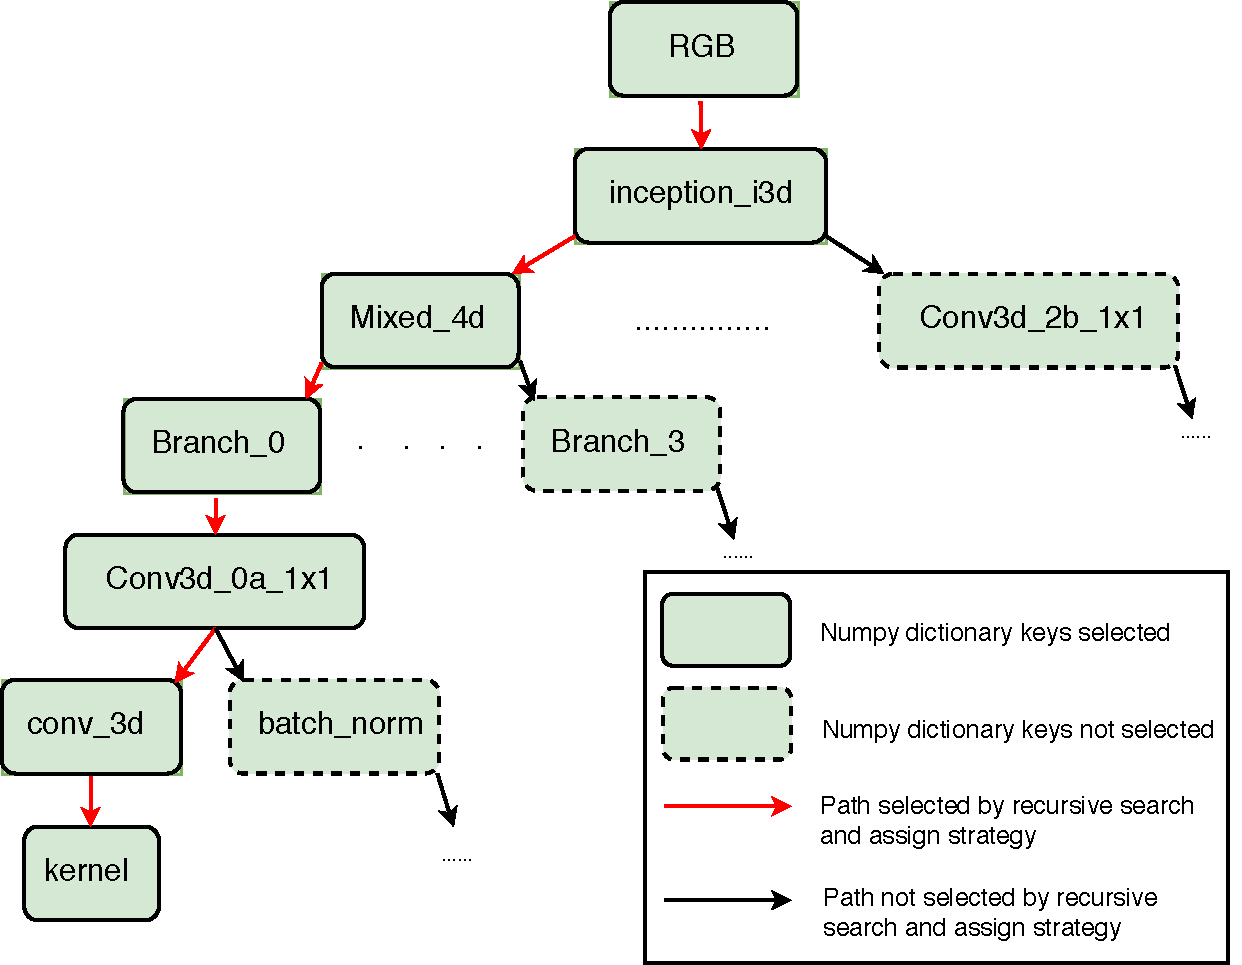
\includegraphics[width=0.7\columnwidth]{images/checkpoint_recursive.pdf}
\caption{The custom numpy dictionary format used to store weights of a model is illustrated here. Each block defines the set of keys available at a particular depth within the numpy final. The leaf block is associated with the final numpy array that is assigned to a tensor whose name can be reconstructured by following the names of each block traversed to reach the leaf block. When initializing a model from a pre-existing dictionary, a depth-first search and assign strategy is used to find and assign tensor values.}
\label{fig:checkpoint_recursive}
\end{figure}
\paragraph{Tensor Handling}
The tensor handler is a recursively defined function which takes names of tensors from the numpy file and loops over assigning the corresponding values associated with those tensor names through the function \texttt{\textcolor{ForestGreen}{tf.assign(tf.graph.get\_tensor\_by\_name(\textless tensor\_name\textgreater), numpy value)}}.
A model is initialized from a pre-existing numpy dictionary through the use of a depth first search and assign policy using the tensor handler.
An example of this is shown in Fig.~\ref{fig:checkpoint_recursive}.

An important rule for the definition of any tensor name is that the name must explicitly use the terms ``\texttt{\textcolor{ForestGreen}{kernel}}'' and ``\texttt{\textcolor{ForestGreen}{bias}}'' to denote the \texttt{W} (weight) and \texttt{b} (bias) matrices respectively.
No other name is recognized within the platform.



\subsection{Metrics Module}
\label{sec:metrics}

\begin{figure}[b!]
\centering
%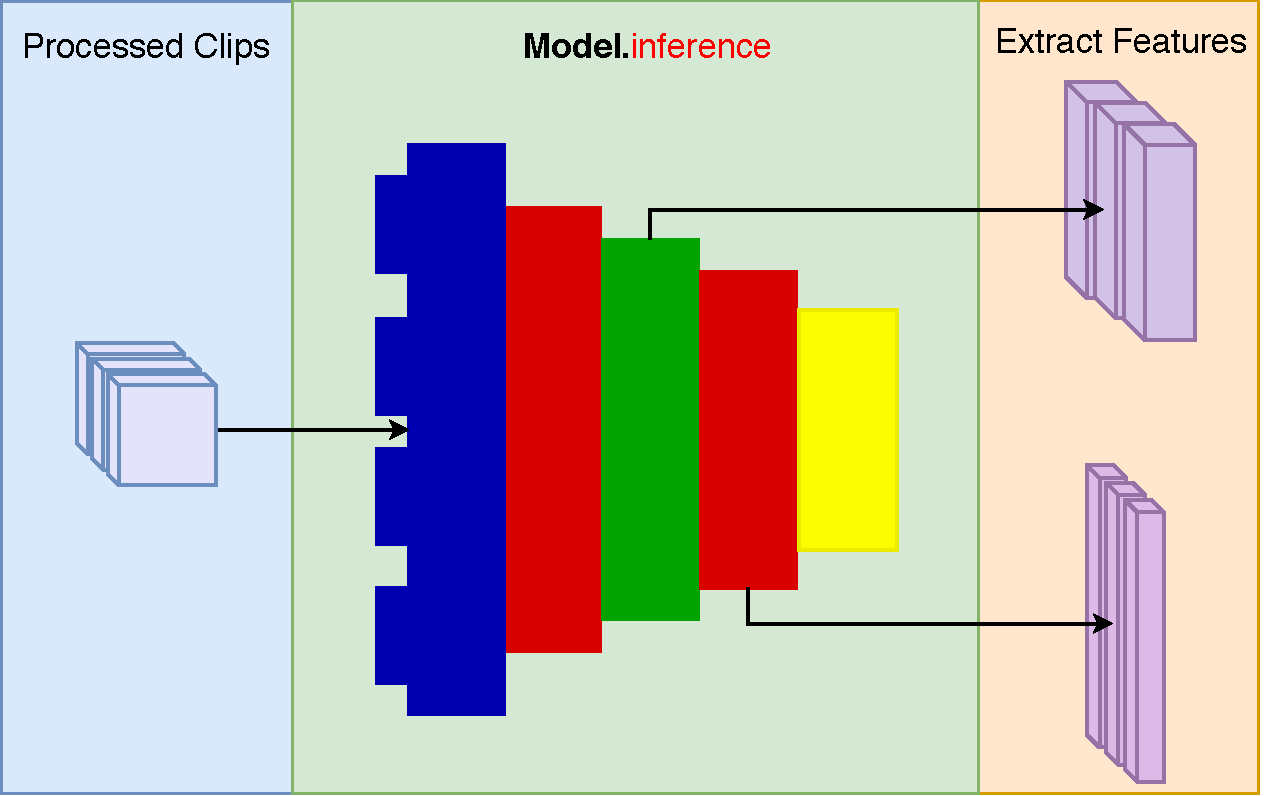
\includegraphics[width=0.7\columnwidth]{images/extract_features_h.pdf}
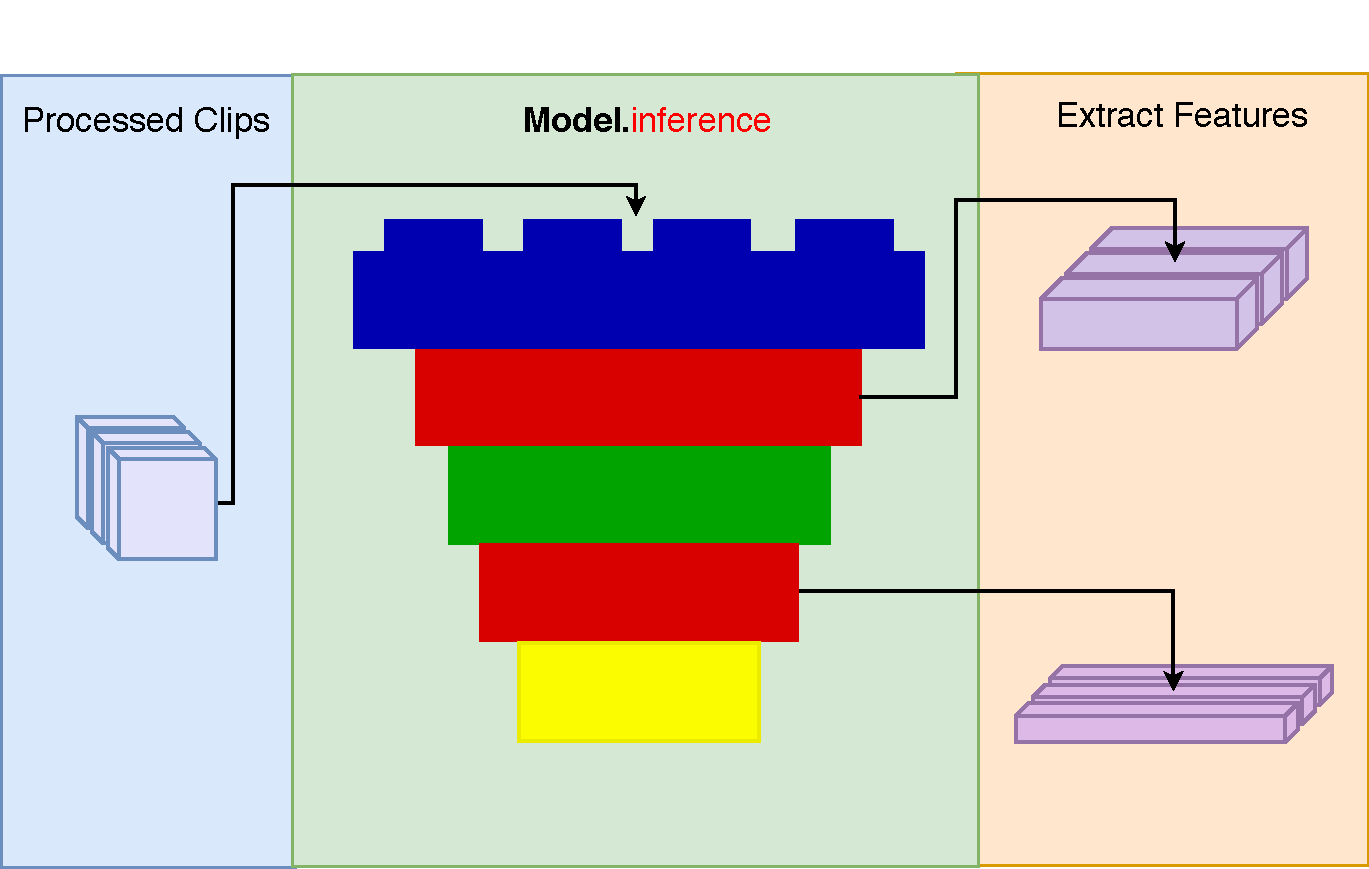
\includegraphics[width=0.7\columnwidth]{images/extract_features.pdf}
\caption{The \metrics utilizes a variety of metrics to measure the performance of a model.
It also allows features to be extracted from any defined model using any appropriately formatted dataset.
This figure conceptualizes the capability of features being extracted from various layers within a model.}
\label{fig:extract_features}
\end{figure}

\acro~offers a \metrics~for testing and logging the activity recognition performance of a model as well as extracting features from a model.
This \metrics~is incorporated in the \textbf{Testing Block} as a class which gets instantiated in \textcolor{blue}{test.py}.
During testing, the model output, correct label, and name of each video gets stored in this \textbf{Metrics} object.
Depending on the layer from which the outputs, either features or predictions, are extracted, they can be too large in size to efficiently store in memory.
Thus all outputs, labels, and names get stored in a temporary hdf5 file format and then deleted at the end of each testing session.
HDF5 files are used due to their quick reading and writing capabilities.
Just before getting deleted, any final video predictions are saved as numpy files if applicable.
Additionally, during testing, the chosen metric and any other specified variable will be logged automatically using tensorboard.

Available performance metrics include average pooling, last frame prediction, and training a linear SVM classifier.
Average pooling is a common technique which uses the softmax per-class predictions of a model and averages them across all frames of an input video.
From these averaged predictions, the arg. maximum value is used as the overall class prediction for that video.
Last frame prediction simply uses the softmax per-class prediction of the last frame in the video to generate the overall class prediction.
Last frame classification is referenced originally in the ConvNet + LSTM model~\cite{donahue2015long}.
In addition to these metrics which directly classify the output of a model, \acro~also provides the option of training a linear SVM classifier based off of features extracted from any user specified layer within the model.
A linear SVM was used to classify videos in the UCF101 dataset in C3D.

Since the output predictions of models can vary in shape so we standardize them to be in the form of [\texttt{\textcolor{ForestGreen}{batch\_size}}, \texttt{\textcolor{ForestGreen}{sequence\_length}}, \texttt{\textcolor{ForestGreen}{number\_of\_classes}}].
The \texttt{\textcolor{ForestGreen}{batch\_size}} parameter slightly changes meaning depending on the model being used.
For example for C3D, it refers to clips extracted from one video that are used for testing which will all get averaged to produce a single video-level prediction.
On the other hand, TSN would take multiple videos and refer to each as a single clip, thus a single batch containing different videos would each be logged separately.
\acro~is robust enough to handle both such cases.

As previously mentioned, \acro~provides the ability to extract features from a model, as shown in Fig.~\ref{fig:extract_features}.
Features can be extracted for a multitude of reasons including to train a linear SVM which allows \acro~to accomplish more than just activity recognition.
Any of the state-of-the-art models that have been implemented, or a custom model, can be used for feature extraction.
With any dataset that has been converted to the proper tfrecords format, the correct input arguments allow the user to extract features from any layer in a given model.
When features are being extracted, the output of a model is not required to be of any standardized form.
Due to the large size that features can become over modern datasets with thousands and even millions of videos, it is crucial to be able to read and write them to memory quickly which is why we use an HDF5 file format for writing this data.




\section{Benchmarks}
\label{sec:benchmarks}
In this section we will be providing numerical evaluations of \acro.

Table \ref{tab:model_results} show the performance on four SOTA models on the HMDB51 and UCF101 datasets.
Results for C3D, I3D, TSN, and ResNet50+LSTM are compared between those generated in \acro~and those given by the original authors of the models.

\begin{table}[h!]
\begin{center}
\caption{Mean recognition accuracies are shown for various SOTA action recognition models across split 1 of HMDB51 and UCF101.
Values marked with a (*) indicate that results are shown across all three splits of a given model.
Accuracies are reported for each baseline model and preprocessing technique combination.}
\label{tab:model_results}
\begin{tabular}{c|c|c|c||c|c}
\hline
\multirow{2}{*}{Base Model} & \multirow{2}{*}{Pretraining} & \multicolumn{2}{c||}{HMDB51 Acc.} & \multicolumn{2}{c}{UCF101 Acc.} \\\cline{3-6}
& & Ours & Authors & Ours & Authors \\
\hline
C3D & Sports-1M & 48.24 & 50.30 * & 93.66 & 82.30 * \\
\hline
I3D & Kinetics & --.-- & 74.80 * & --.-- & 95.60 * \\
\hline
TSN & ImageNet & 51.70 & 54.40 & 85.25 & 85.50 \\
\hline
ResNet50+LSTM & ImageNet & 43.86 & 43.90 & 80.20 & 84.30 \\
\hline
\end{tabular}
\end{center}
\end{table}


\subsection{C3D}
\label{sec:c3d}

Table \ref{tab:c3d} shows more detailed results of the various finetuining methods used for C3D on split 1 of HMDB51 and UCF101.
C3D~\cite{} was originally trained on the Sports-1M~\cite{} dataset, then used on other activity recognition datasets by exctracting C3D features and training a linear SVM for activity classification.
Most models are transferred to a new dataset by finetuneing either the entire model or a select few layers on the new dataset in order to incorporate a different number of action classes.
In the paper introducing Res3D~\cite{}, the authors give results for the original C3D model architecture finetuned on HMDB51 and UCF101.
Code is available for both the original C3D feature extraction method as well as the finetuning method, however it is entirely in Caffe.
In order to use the available models, they first need to be converted to tensorflow, which was done by GitHub user hx173149\footnote{https://github.com/hx173149/C3D-tensorflow}.
This tensorflow version of C3D provides the original Sports-1M trained model as well as the weights after fine-tuning it on UCF101.
While this tensorflow implementation is slightly different than that used in \acro, we will be using these weights to compare C3D performance on UCF101.
Minor variations include the use of the Sport-1M mean clip in our implementation versus the UCF101 mean clip.
Our other models are generally all pre-trained on the ImageNet~\cite{} dataset and use the ImageNet mean image to normalize their data.
For this reason, we use the Sports-1M mean clip to normalize C3D data since it was pre-trained on that dataset, as opposed to the UCF101 mean clip which we finetune on.
This makes it easier to add new datasets since the same Sports-1M mean clip file will be used for fine-tuning in all cases.

No weights are available for C3D that have been finetuned on HMDB51, thus we finetune it entirely in \acro~from the provided Sports-1M model.



\begin{table}[h!]
\begin{center}
\label{tab:c3d}
\caption{Mean recognition accuracies are shown for C3D finetuned on split 1 of HMDB51 and UCF101.
Values marked with a (*) indicate that results are shown across all three splits of a given model.
The "Training" column denotes which datasets were used to achieve the given performance.
All models were intially train on Sports-1M in Caffe by the authors of C3D.
This model was converted to tensorflow and then we finetune directly on it within \acro~for HMDB51.
There exists a model in the tensorflow version of C3D which was the original Sports-1M model then finetuned on UCF101.
We attempt to use these weights directly to match the reported clip-accuracy.
We also use these UCF101 finetune weights and finetune on them more within \acro.
We report results after one and ten additional epochs of finetuning within \acro.}
\label{tab:model_results}
\begin{tabular}{c|c|c|c}
\hline
\multirow{2}{*}{Base Model} & \multirow{2}{*}{Training} & \multicolumn{2}{c}{HMDB51 Acc.} \\\cline{3-4}
& & Ours & Authors\\
\hline
C3D & Sport1M \footnote{We finetune the Sports-1M trained model of C3D found at https://github.com/hx173149/C3D-tensorflow under Download: "C3D sports1M". The file is named conv3d\_deepnetA\_sport1m\_iter\_1900000\_TF.model and renamed to c3d\_Sports1M.npy in \acro.} + 41 Epochs HMDB51 in \acro & 48.24 & 50.30 *\\ 
\hline
\\[-0.2 cm]
\hline
\multirow{1}{*}{} & \multirow{1}{*}{} & \multicolumn{2}{c}{UCF101 Acc.} \\
\hline
C3D & Sports-1M + UCF101 & 73.46 & 74.65\footnote{This is the tensorflow version of C3D trained on Sports-1M and finetuned on UCF101 which achieved a clip-accuracy of 74.65\%. We are testing directly on the provided weights found under Download: "C3D UCF101 split1" at https://github.com/hx173149/C3D-tensorflow. The file is named sports1m\_finetuning\_ucf101.model and in \acro~we renamed it to c3d\_Sports1M\_finetune\_UCF101.npy. Since we are directly using these weights, we try to match 74.65\% even though the original authors achieved 82.30\%.} \\
\hline
C3D & Sports-1M + UCF101 + 1 Epoch UCF101 in \acro & 91.04 & 74.65 \\
\hline
C3D & Sports-1M + UCF101 + 10 Epochs UCF101 in \acro & 93.66 & 74.65 \\
\hline
\end{tabular}
\end{center}
\end{table}











%\section{Future Endeavors}
%\label{sec:future}



\clearpage

\bibliographystyle{splncs}
\bibliography{egbib}

\end{document}

\grid
\grid
\grid
\grid
\grid
